\documentclass[prb,aps,twocolumn,showpacs,10pt]{revtex4-1}
\pdfoutput=1
\usepackage{dcolumn}% Align table columns on decimal point
\usepackage{bm}% bold math

%\usepackage{anysize}
\usepackage[colorlinks,hyperindex, urlcolor=blue, linkcolor=blue,citecolor=black, linkbordercolor={.7 .8 .8}]{hyperref}
\usepackage{graphicx}
%\usepackage{tabularx}
\usepackage{amsfonts}
\usepackage{amsmath}
\usepackage{amssymb}
\usepackage{amsbsy}
\usepackage{tikz}
\usepackage{caption}
\usepackage{subcaption}
\usepackage{nicefrac}
\usetikzlibrary{arrows,shapes,positioning}
\newenvironment{psmallmatrix}
  {\left[\begin{matrix}}
  {\end{matrix}\right]}
\usetikzlibrary{arrows,shapes,positioning}
\usetikzlibrary{decorations.markings}
  
 \usepackage{listings}
\usepackage{color}

\definecolor{dkgreen}{rgb}{0,0.6,0}
\definecolor{gray}{rgb}{0.5,0.5,0.5}
\definecolor{mauve}{rgb}{0.58,0,0.82}

\lstset{frame=tb,
  language=Java,
  aboveskip=3mm,
  belowskip=3mm,
  showstringspaces=false,
  columns=flexible,
  basicstyle={\small\ttfamily},
  numbers=none,
  numberstyle=\tiny\color{gray},
  keywordstyle=\color{blue},
  commentstyle=\color{dkgreen},
  stringstyle=\color{mauve},
  breaklines=true,
  breakatwhitespace=true,
  tabsize=3
}


\newcommand{\etal}{{\it et~al.}}

\graphicspath{{figures/}}

\begin{document}

\title {Project 4: Modeling the Spread of an Infectious Disease}

\author{Jane Kim}
\affiliation{Physics 480: Computational Physics}
\date{\today}


\begin{abstract}
\vspace*{3mm}
A Monte Carlo simulation of the spread of an infectious disease in an isolated population was constructed from the SIRS model. Four populations (A,B,C, and D) with different rates of recovery were studied and compared to the predictions from a deterministic approximation. One hundred samples were generated for each population, which was enough to produce relatively smooth averages but varying standard deviations. Larger uncertainties were observed in populations B and C due to the enhanced nonlinearity of the system.
\end{abstract}

\maketitle

\section{Introduction}

The goal of this project was to develop a Monte Carlo simulation of the spread of an infectious disease. The classical SIRS model of epidemiology was studied and used to develop the necessary transition probabilities for the simulation. Interpreting the simulation requires a thorough understanding of the SIRS model, so a deterministic approach was used in conjunction with the Monte Carlo methods. \\

The main purpose of creating such a simulation is to investigate how a disease spreads throughout a given population over time. Then we can make predictions about whether or not a certain disease has the capacity to establish itself within the population, i.e. a fraction of the population remains infected after the system reaches equilibrium. \\

In the following section, the SIRS model is discussed in-depth. Then in Section III, the SIRS model is adapted for the Monte Carlo simulation and four test cases are described. The implementation of the SIRS model using both deterministic and stochastic approaches is presented in Section IV, the results of which are shown in Section V. Finally, possible improvements upon the model are described in Section VI and the conclusion is given in Section VII.\\


\section{Theory}
The SIRS model considers an isolated population of $N$ people which are divided into three separate groups: 
\begin{itemize}
\item Susceptible (S): those without immunity to the disease,
\item Infected (I): those who are currently infected with the disease,
\item Recovered (R): those who have been infected in the past and have developed an immunity to the disease.
\end{itemize}
A person can move from one group to another only in the cyclic order suggested by the name of the model $S\rightarrow I \rightarrow R \rightarrow S$. The rate of transmission $a$, the rate of recovery $b$ and the rate of immunity loss $c$ help describe the flow of people moving between the three groups. The population is assumed to mix homogeneously and total population is assumed to remain constant so that
\begin{equation}
N = S(t)+I(t)+R(t).
\end{equation} 
For the simple case, we will assume that the dynamics of the epidemic occur during a time scale much smaller than the average person's lifetime. Hence the effect of the birth and death rate of the population is ignored.\\

From these assumptions, a set of coupled differential equations can be constructed to form the classical SIRS model:
\begin{equation}
\begin{split}
S'&=cR-\frac{aSI}{N}\\
I'&=\frac{aSI}{N}-bI\\
R'&=bI-cR\\
\end{split}
\end{equation}
Note that for small populations, one may choose to write $aSI$ instead of $\frac{aSI}{N}$ since the number of susceptibles which become infected depend more on the absolute number of infected people rather than the infected fraction of the population.\\

Though this set does not have analytic solutions like the closely-related SIR model, the equilibrium solutions are simple to obtain. The constraint in (1) reduces this three dimensional system into a two dimensional one so that the equation for $R'$ can just be omitted:
\begin{equation}
\begin{split}
S'&=c(N-S-I)-\frac{aSI}{N}\\
I'&=\frac{aSI}{N}-bI\\
\end{split}
\end{equation}
The steady state is found by setting both equations in (3) equal to zero. Let $s$, $i$, and $r$ denote the fractions of people in $S$, $I$, and $R$, respectively. Then the fractions of people in each group at equilibrium are:
\begin{equation}
\begin{split}
s^* &= \frac{b}{a},\\
i^* &= \frac{1-\frac{b}{a}}{1+\frac{b}{c}},\\
r^* &= \frac{b}{c}\frac{1-\frac{b}{a}}{1+\frac{b}{c}}.
\end{split}
\end{equation}
Here, the asterisk ($^*$) signifies that these fractions are at equilibrium. Notice that each fraction must be a number between 0 and 1, and that the three fractions must add up to 1. Thus the equations in (4) suggest that the rate of recovery $b$ must be less than the rate of transmission $a$ for the number of infected people at equilibrium to be greater than zero. In other words, the disease establishes itself in the population only if $b<a$. \\


\section{Method}
Four different populations were created to investigate the effect of increasing the rate of recovery $b$ and crossing the "threshold". Each population consisted of 400 people, 100 of which were initially infected and 300 of which were initially susceptible. The rate of transmission $a$ and the rate of immunity loss $c$ were consistent between populations, but the rate of recovery $b$ was varied because it is the one parameter which can be reasonably controlled by the actions of human society (access to health care, development of new medicines, etc). Note that the rates have units of inverse time. \\
\begin{center}
\begin{tabular}{|c|c|c|c|c|}
\hline
\textbf{Rate}&\textbf{A}&\textbf{B}&\textbf{C}&\textbf{D}\\
\hline
\hline
a&4&4&4&4\\
\hline
b&1&2&3&4\\
\hline
c&0.5&0.5&0.5&0.5\\
\hline
\end{tabular}
\vspace*{5mm}

Table 1: Rates of transmission $a$, recovery $b$, and immunity loss $c$ for populations $A$, $B$, $C$, and $D$.
\end{center}

\vspace*{5mm}
The set of differential equations in (2) inherently assume that $S$, $I$, and $R$ are continuous variables, when they are discrete in reality. We can use the idea of randomness to remedy this issue by defining a set of transition probabilities for the possible moves a person can take from one state to another: $S\rightarrow I$, $I \rightarrow R$, and $R \rightarrow S$. To obtain the specific values for each probability, we first notice from (2) that in a small time step $\Delta t$, the number of people moving from $S$ to $I$ is approximately $\frac{aSI}{N}\Delta t$. Likewise, about $bI\Delta t$ move from $I$ to $R$ and $cR\Delta t$ move from $R$ to $S$. \\

Now we let $\Delta t$ be small enough so that \textit{at most} one person moves from a given group to another. Since
\begin{equation}
\begin{split}
&\max \Big\{ \frac{aSI}{N}\Delta t \Big\} = \frac{a}{N}\left(\frac{N}{2}\right)^2\Delta t=\frac{aN}{4}\Delta t,\\
&\max \Big\{ bI\Delta t \Big\} = bN\Delta t,\\
&\max \Big\{ cR\Delta t \Big\} = cN\Delta t,\\
\end{split}
\end{equation}
the time step is then given by
\begin{equation}
\Delta t = \min \Big\{ \frac{4}{aN}, \frac{1}{bN}, \frac{1}{cN} \Big\}.
\end{equation}
This construction allows us to reinterpret the values $\frac{aSI}{N}\Delta t$, $bI\Delta t$, and $cR\Delta t$ as transition probabilties:
\begin{equation}
\begin{split}
P(S\rightarrow I) &= \frac{aSI}{N}\Delta t,\\
P(I \rightarrow R) &= bI\Delta t,\\
P(R \rightarrow S) &= cR\Delta t.\\
\end{split}
\end{equation}
For each possible move, a random number between 0 and 1 is generated. If the number is less than the probability for the move, the move is taken.\\


\section{Implementation}

A class called \texttt{CInfectedPopulation} was created to carry the parameters $N$, $a$, $b$, and $c$ for each population. Then its member functions \texttt{deterministic\_SIRS} and \texttt{montecarlo\_SIRS} solve the system with a deterministic and Monte Carlo approach, respectively. Both functions require a file name and initial conditions, and the latter also requires a number of samples \texttt{nsamples}.\\

\subsection{Deterministic Approximation}

The function \texttt{deterministic\_SIRS} solves the system of differential equations in (2) using the second order Runge-Kutta formula. The number of people in each category are then written to file at each time step.
\begin{lstlisting}
void CInfectedPopulation::deterministic_SIRS(string filename, double S0, double I0, double tf){

	// open file
	ofstream outfile;
	outfile.open(filename + ".dat");
	cout << "write to ---> " << "'" << filename+".dat'" << endl;

	// file headings
	outfile << "# N = " << N_ << endl;
	outfile << "# (S0, I0, R0) = (" << S << ", " << I << ", " << R << ")" << endl;
	outfile << "# (a, b, c) = (" << a_ << ", " << b_ << ", " << c_ << ")" << endl;
	outfile << "# time, S, I, R" << endl;


	// initial conditions
	double S = S0, I = I0, R = N_-S0-I0;
	double S_k1, S_k2, I_k1, I_k2, R_k1, R_k2;
	
	for(double t = 0.0; t < tf; t += dt_){

		// print 
		outfile << t << "\t" << S << "\t" << I << "\t" << R << endl;

		// use RK2 method to calculate next S, I, R
		S_k1 = dt_*(c_*R-a_*S*I/N_);
		I_k1 = dt_*(a_*S*I/N_-b_*I);
		R_k1 = dt_*(b_*I-c_*R);

		S_k2 = dt_*(c_*(R+0.5*R_k1) -a_*(S+0.5*S_k1)*(I+0.5*I_k1)/N_);
		I_k2 = dt_*(a_*(S+0.5*S_k1)*(I+0.5*I_k1)/N_ -b_*(I+0.5*I_k1));
		R_k2 = dt_*(b_*(I+0.5*I_k1) -c_*(R+0.5*R_k1));

		S += S_k2;
		I += I_k2;
		R += R_k2;
	}
	// close file
	outfile.close();
}
\end{lstlisting}
A phase portrait was generated for each population by running the above function with various initial conditions and plotting $S$ vs. $I$ as the system evolves over time.

\subsection{Monte Carlo Simulation}

The vast majority of \texttt{montecarlo\_SIRS} is devoted to calculating the averages and standard deviations of the \texttt{nsamples} samples for each time step. Only three simple lines within a loop is required to actually run the simulation. Hence it is quite quick and easy to obtain the results.
\begin{lstlisting}
void CInfectedPopulation::montecarlo_SIRS(string filename, int nsamples, int S0, int I0, double tf){

	// RNG
	mt19937 generator;
	uniform_real_distribution<double> rand01(0.0, 1.0);

	// time vector
	vector<double> time;
	for(double t = 0.0; t < tf; t += dt_) time.push_back(t);
	int ntimes = time.size();
	
	// averages for each point in time
	vector<double> avgS(ntimes,0.0), avgI(ntimes,0.0), avgR(ntimes,0.0);

	// create random samples
	for(int n = 0; n < nsamples; ++n){

		// open file
		ofstream outfile;
		outfile.open(filename+to_string(n)+".dat");
		cout << "write to ---> " << "'" << filename+to_string(n)+".dat'" << endl;

		// file headings
		outfile << "# N = " << N_ << endl;
		outfile << "# (S0, I0, R0) = (" << S << ", " << I << ", " << R << ")" << endl;
		outfile << "# (a, b, c) = (" << a_ << ", " << b_ << ", " << c_ << ")" << endl;
		outfile << "# time, S, I, R" << endl;

		// initial conditions
		int S = S0, I = I0, R = N_-S0-I0;

		// run simulation
		for(int i = 0; i < ntimes; ++i){

			// write to file
			outfile << time[i] << "\t" << S << "\t" << I << "\t" << R << endl;
			
			// calculate averages
			avgS[i] += S/(double) nsamples;
			avgI[i] += I/(double) nsamples;
			avgR[i] += R/(double) nsamples;

			// keep-or-reject
			if(rand01(generator) < a_*S*I*dt_/N_){ I += 1; S -= 1; }
			if(rand01(generator) < b_*I*dt_){ R += 1; I -= 1; }
			if(rand01(generator) < c_*R*dt_){ S += 1; R -= 1; }
		}
		outfile.close();
	}

	double t, S, I, R;
	double avg_sigS = 0.0, avg_sigI = 0.0, avg_sigR = 0.0;
	string dummy;
	vector<double> varS(ntimes,0.0);
	vector<double> varI(ntimes,0.0);
	vector<double> varR(ntimes,0.0);
	int count = 0;

	// calculate variances
	for(int n = 0; n < nsamples; ++n){

		ifstream infile;
		infile.open(filename + to_string(n) + ".dat");


		// ignore headings
		for(int i = 0; i < 4; ++i) getline(infile, dummy);

		// calculate variance and average standard deviation
		for(int i = 0; i < ntimes; ++i){

			infile >> t >> S >> I >> R;

			varS[i] += (avgS[i]-S)*(avgS[i]-S)/(nsamples-1);
			varI[i] += (avgI[i]-I)*(avgI[i]-I)/(nsamples-1);
			varR[i] += (avgR[i]-R)*(avgR[i]-R)/(nsamples-1);

			avg_sigS += sqrt(varS[i])/(nsamples*ntimes);
			avg_sigI += sqrt(varI[i])/(nsamples*ntimes);
			avg_sigR += sqrt(varR[i])/(nsamples*ntimes);
		}

		infile.close();
	}

	// write averages and standard deviations to file
	ofstream outfile;
	outfile.open(filename+to_string(nsamples) +"_stats.dat");
	cout << "write to ---> " << "'" << filename+to_string(nsamples) +"_stats.dat" << endl;

	outfile << "# N = " << N_ << endl;
	outfile << "# nsamples = " << nsamples << endl;
	outfile << "# (S0, I0, R0) = (" << S0 << ", " << I0 << ", " << N_-S0-I0 << ")" << endl;
	outfile << "# (a, b, c) = (" << a_ << ", " << b_ << ", " << c_ << ")" << endl;
	outfile << "# time avg std dev (<sigma S>, <sigma I>, <sigma R>) = (" << avg_sigS << ", " << avg_sigI << ", " << avg_sigR << ")" << endl;
	outfile << "# time, avg S, sigma S, avg I, sigma I, avg R, sigma R" << endl;

	for(int i = 0; i < ntimes; ++i){
		outfile << time[i] << "\t" << avgS[i] << "\t" << sqrt(varS[i]);
		outfile << "\t" << avgI[i] << "\t" << sqrt(varI[i]);
		outfile << "\t" << avgR[i] << "\t" << sqrt(varR[i]) << endl;
	}

	outfile.close();
}
\end{lstlisting}

\section{Results}

Based on (4) and our choices of parameters in Table 1, the fractions of people at equilibrium in each category is as follows:
\begin{center}
\begin{tabular}{|c|c|c|c|c|}
\hline
\textbf{Fraction}&\textbf{A}&\textbf{B}&\textbf{C}&\textbf{D}\\
\hline
\hline
$s^*$&1/4&1/2&3/4&1\\
\hline
$i^*$&1/4&1/10&1/28&0\\
\hline
$r^*$&1/2&2/5&3/14&0\\
\hline
\end{tabular}
\vspace*{5mm}

Table 2: The expected fractions of people in each category at equilibrium for populations $A$, $B$, $C$, and $D$.
\end{center}
\vspace*{5mm}
These fractions provide a useful test for both approaches to solving the SIRS model.


\subsection{Deterministic Approximation}
The number of people in each category is plotted in Figure 1 for all four populations. As expected, the number of infected people drops as the rate of recovery increases. However, the population becomes vulnerable to an outbreak when the rate of recovery equals the rate of transmission (population D) because the entire population eventually becomes susceptible. \\

The phase portraits for each population are shown in Figure 2. Since the total population is assumed to be constant, the area above the dashed lines are inaccessible. In general, the solutions spiral toward a stable equilibrium point located somewhere within the boundaries of the triangle or at (s,i)=(1,0). Notice that for populations $B$ and $C$, the spirals are confined to a smaller region in phase space, leading to large changes in one variable and small changes in the other. \\

\subsection{Monte Carlo Simulation}

One hundred samples were generated for each population and plotted in Figure 3. This was enough to produce smooth averages, but the average for population $C$ did not agree with the deterministic approximation. For example, the fraction of people in the susceptible category appeared to tend to 1 rather than 3/4.\\

The standard deviations are relatively small for populations $A$ and $D$, but large for $B$ and $C$. This may be due to the exaggerated nonlinearity found in the phase portraits for these populations. The time-averaged standard deviations for each population are:
\begin{center}
\begin{tabular}{|c|c|c|c|c|}
\hline
&A&B&C&D\\
\hline
\hline
$\langle \sigma_S \rangle$ &7.095&16.56&20.98&3.492\\
\hline
$\langle \sigma_I \rangle$&6.716&7.561&4.075&0.651\\
\hline
$\langle \sigma_R \rangle$&5.892&12.73&17.89&3.221\\
\hline
\end{tabular}
\end{center}
Compared to the population size of $N=400$, the differences between populations are significant.

\section{Improvements}
The same principles used in this simple model can be extended to include more details about the population and disease.
\subsection{Vital Dynamics}
For instance, vital dynamics can be easily added to the system so that the model can describe the spread of diseases which occur over longer stretches of time. If $b$ is the birth rate, $d$ is the death rate, and $d_I$ is the death rate of infected people due to the disease, then the modified differential equations are given by:
\begin{equation}
\begin{split}
S'&=cR-\frac{aSI}{N}-dS+eN\\
I'&=\frac{aSI}{N}-bI-dI-d_I I\\
R'&=bI-cR-dR\\
\end{split}
\end{equation}
Here, we have assumed that all the babies born into the population are initially susceptible. 

\subsection{Seasonal Variation}

For diseases such as influenza, the rate of transmission depends largely on the time of year. During the colder months, individuals are more likely to spend time in closer proximity to one another, resulting in a rate of transmission which oscillates. So we can let $a$ be given by
\begin{equation}
a(t)=Acos(\omega t) + a_0,
\end{equation}
where $a_0$ is the average transmission rate, $A$ is the maximum deviation from $a_0$, and $\omega$ is the frequency of oscillation.\\

\subsection{Vaccination}

Diseases with available vaccinations allow people to move directly from $S$ to $R$, breaking the cyclic structure of the SIRS model. We assume that a susceptible individual's choice to become vaccinated does not depend on how many other susceptibles are vaccinated. We may, however, assume that the rate of vaccination $f$ can depend on the time, since this rate may oscillate during the course of a year and/or increase as awareness and medical research increases. Then the system of differential equations become
\begin{equation}
\begin{split}
S'&=cR-\frac{aSI}{N}-f\\
I'&=\frac{aSI}{N}-bI\\
R'&=bI-cR+f\\
\end{split}
\end{equation}

\subsection{Inhomogeneity}

A major flaw of the SIRS model is that the population is assumed to mix homogeneously. This is not at all realistic, since we all know from experience that it is more likely for people to infect others that come into contact with them, either directly or indirectly. So we can instead develop a spatial model for the spread of a disease using the same compartmental design of the SIRS model. \\

We can start by creating a square lattice with $N$ lattice sites. We randomly place $I_0$ infected people and $R_0$ recovered people on the lattice, and filling the remaining lattice sites with susceptibles. Then at each time step, a random infected site is chosen from a list and recovered with probability $\beta$. Next, one of its nearest neighbors (with periodic boundary conditions) is randomly chosen and infected with probability $\alpha$. Finally, a recovered site is randomly chosen from another list and becomes susceptible with probability $\gamma$.\\

These transition probabilities $\alpha$, $\beta$, and $\gamma$ are different from (7) since equations (2) no longer apply. A simple alternative would just depend on the rates, such as:
\begin{equation}
\begin{split}
\alpha &= \frac{a}{a+b+c} = P(S\rightarrow I)\\
\beta &= \frac{b}{a+b+c} = P(I\rightarrow R)\\
\gamma &= \frac{c}{a+b+c} = P(R\rightarrow S)\\
\end{split}
\end{equation}


\section{Conclusion}

Overall, the results of the Monte Carlo simulation closely  followed the deterministic approximations when the critical point of the phase portrait (Figure 2) was either far from the boundary or on the boundary itself. When it was near the boundary, the heightened nonlinearity caused the spread of the samples to significantly rise.\\

The SIRS model is an excellent starting point for modeling the spread of an infectious disease. As shown in the previous section, additional details can be added later on to match the specifics of a given disease and/or population. A major drawback of the model, however, is that the population is assumed to mix homogeneously. Therefore, the development of a spatial model is recommended. \\



 
\begin{center}
\begin{figure*}
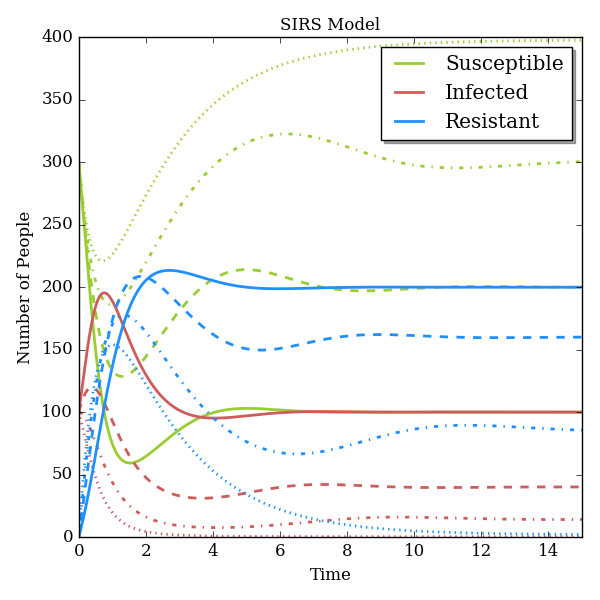
\includegraphics[scale=0.8]{SIR_t.png}
\caption{The number of people in each category for all populations $A$ (solid), $B$ (dashed), $C$ (dot-dashed), and $D$ (dotted).}
\end{figure*}
\end{center}

\begin{figure*}
\centering
\begin{subfigure}{.5\textwidth}
  \centering
  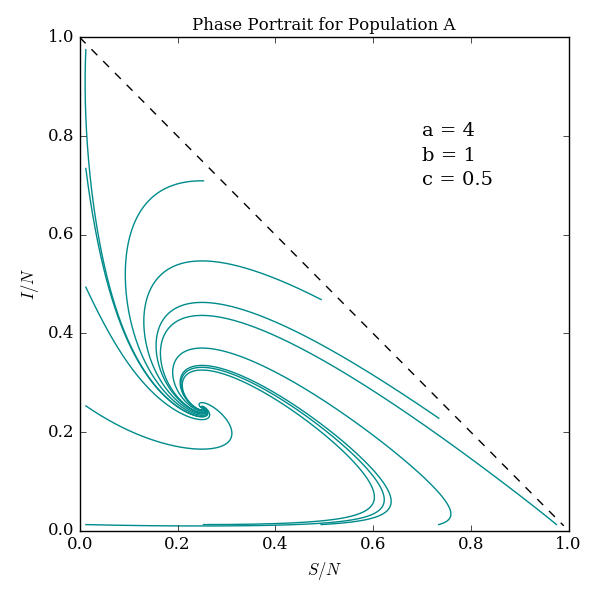
\includegraphics[width=\linewidth]{phaseportrait_A.png}
  \label{fig:sub1}
\end{subfigure}%
\begin{subfigure}{.5\textwidth}
  \centering
  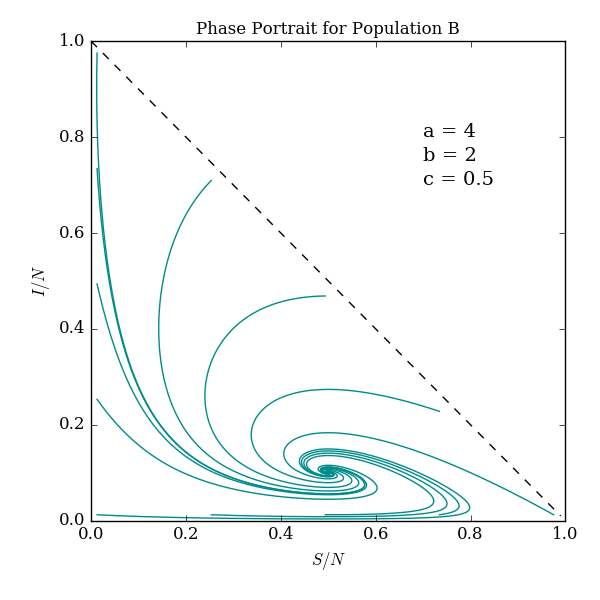
\includegraphics[width=\linewidth]{phaseportrait_B.png}
  \label{fig:sub2}
\end{subfigure}
\label{fig:test}

\medskip
\centering
\begin{subfigure}{.5\textwidth}
  \centering
  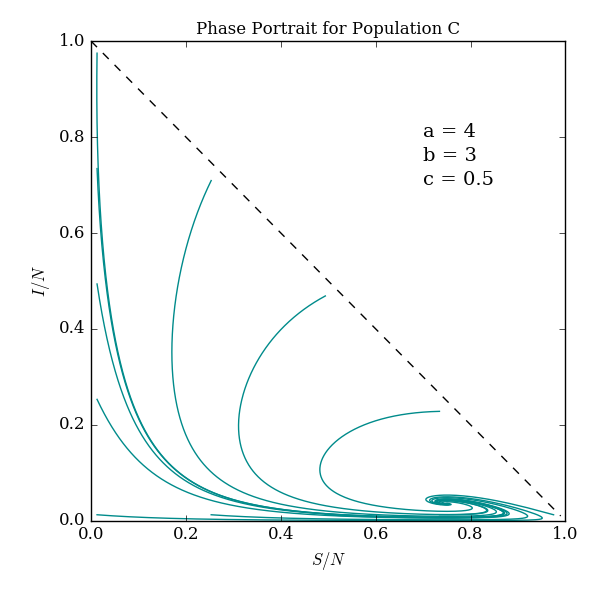
\includegraphics[width=\linewidth]{phaseportrait_C.png}
  \label{fig:sub1}
\end{subfigure}%
\begin{subfigure}{.5\textwidth}
  \centering
  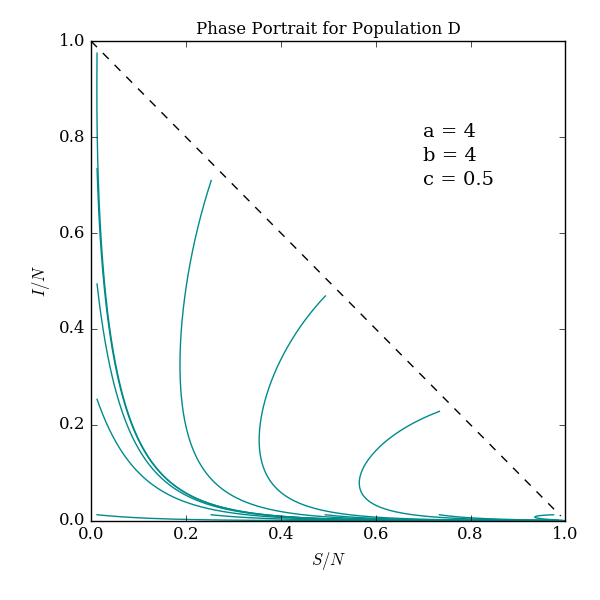
\includegraphics[width=\linewidth]{phaseportrait_D.png}
  \label{fig:sub2}
\end{subfigure}
\label{fig:test}
\caption{Phase portraits for all populations A, B, C, and D.}
\end{figure*}

\begin{figure*}
\centering
\begin{subfigure}{.5\textwidth}
  \centering
  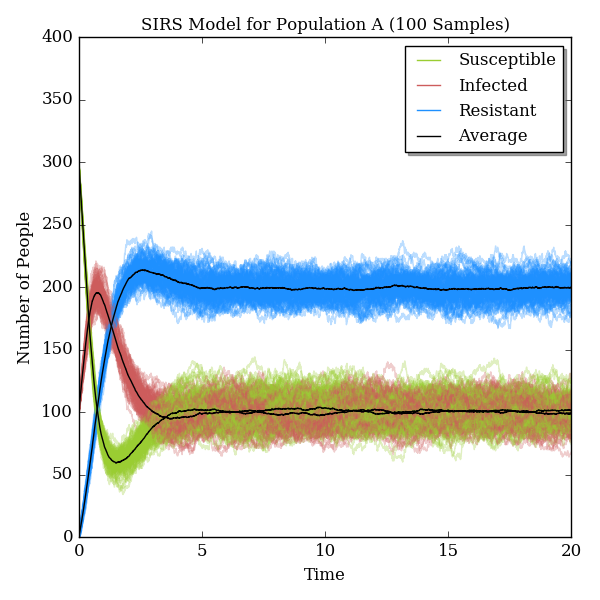
\includegraphics[width=\linewidth]{trials_A100.png}
  \label{fig:sub1}
\end{subfigure}%
\begin{subfigure}{.5\textwidth}
  \centering
  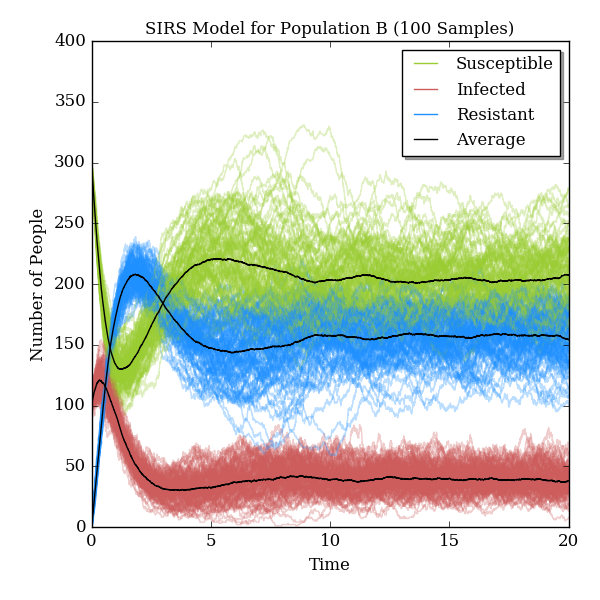
\includegraphics[width=\linewidth]{trials_B100.png}
  \label{fig:sub2}
\end{subfigure}
\label{fig:test}

\medskip
\centering
\begin{subfigure}{.5\textwidth}
  \centering
  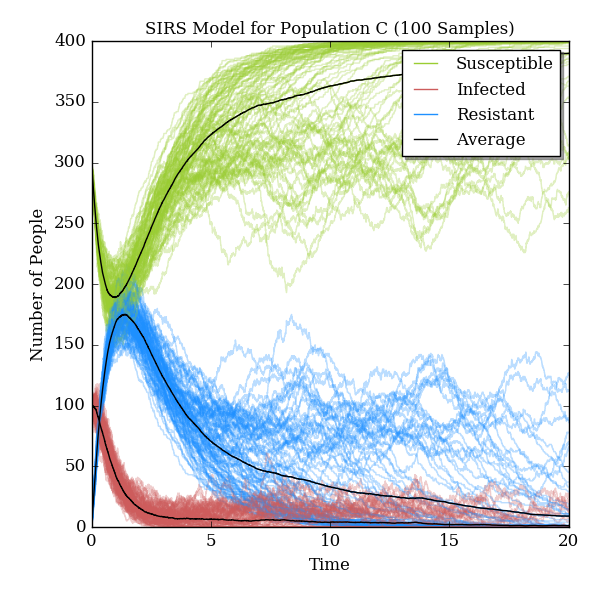
\includegraphics[width=\linewidth]{trials_C100.png}
  \label{fig:sub1}
\end{subfigure}%
\begin{subfigure}{.5\textwidth}
  \centering
  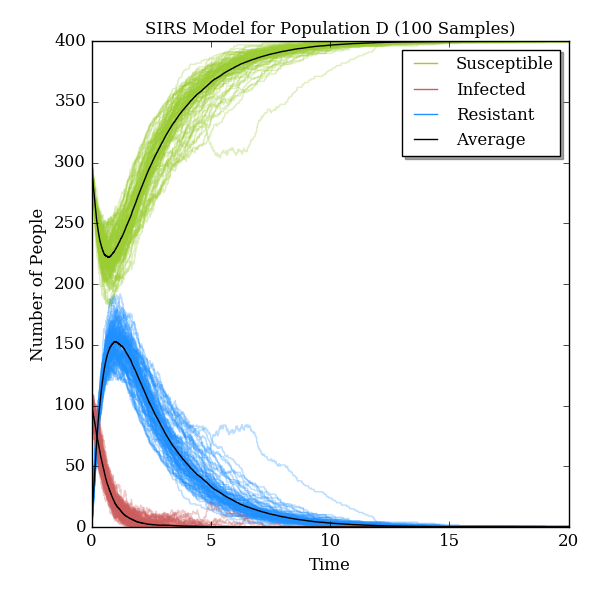
\includegraphics[width=\linewidth]{trials_D100.png}
  \label{fig:sub2}
\end{subfigure}
\label{fig:test}
\caption{Monte Carlo simulation with 100 samples for all populations A, B, C, and D.}
\end{figure*}




\begin{references}
\bibitem{notes} M. Hjorth-Jensen. "Computation Physics, Lecture Notes Fall 2015". University of Oslo. August 2015.
\bibitem{sirs} \url{http://leonidzhukov.net/hse/2014/socialnetworks/papers/2000SiamRev.pdf}
\end{references}

\end{document}
